\chapter{Schnittstellen}

Das Aufnahmesystem kommuniziert sowohl mit dem TourLive Server als auch mit dem Device Management Server in beide Richtungen. In diesem Kapitel werden die Schnittstellen zwischen Aufnahmesystem, TourLive Server sowie Device Management Server und die öffentliche Schnittstelle erläutert. Die folgende Graphik gibt einen Überblick über alle Schnittstellen.

\begin{figure}[H]
	\centering
	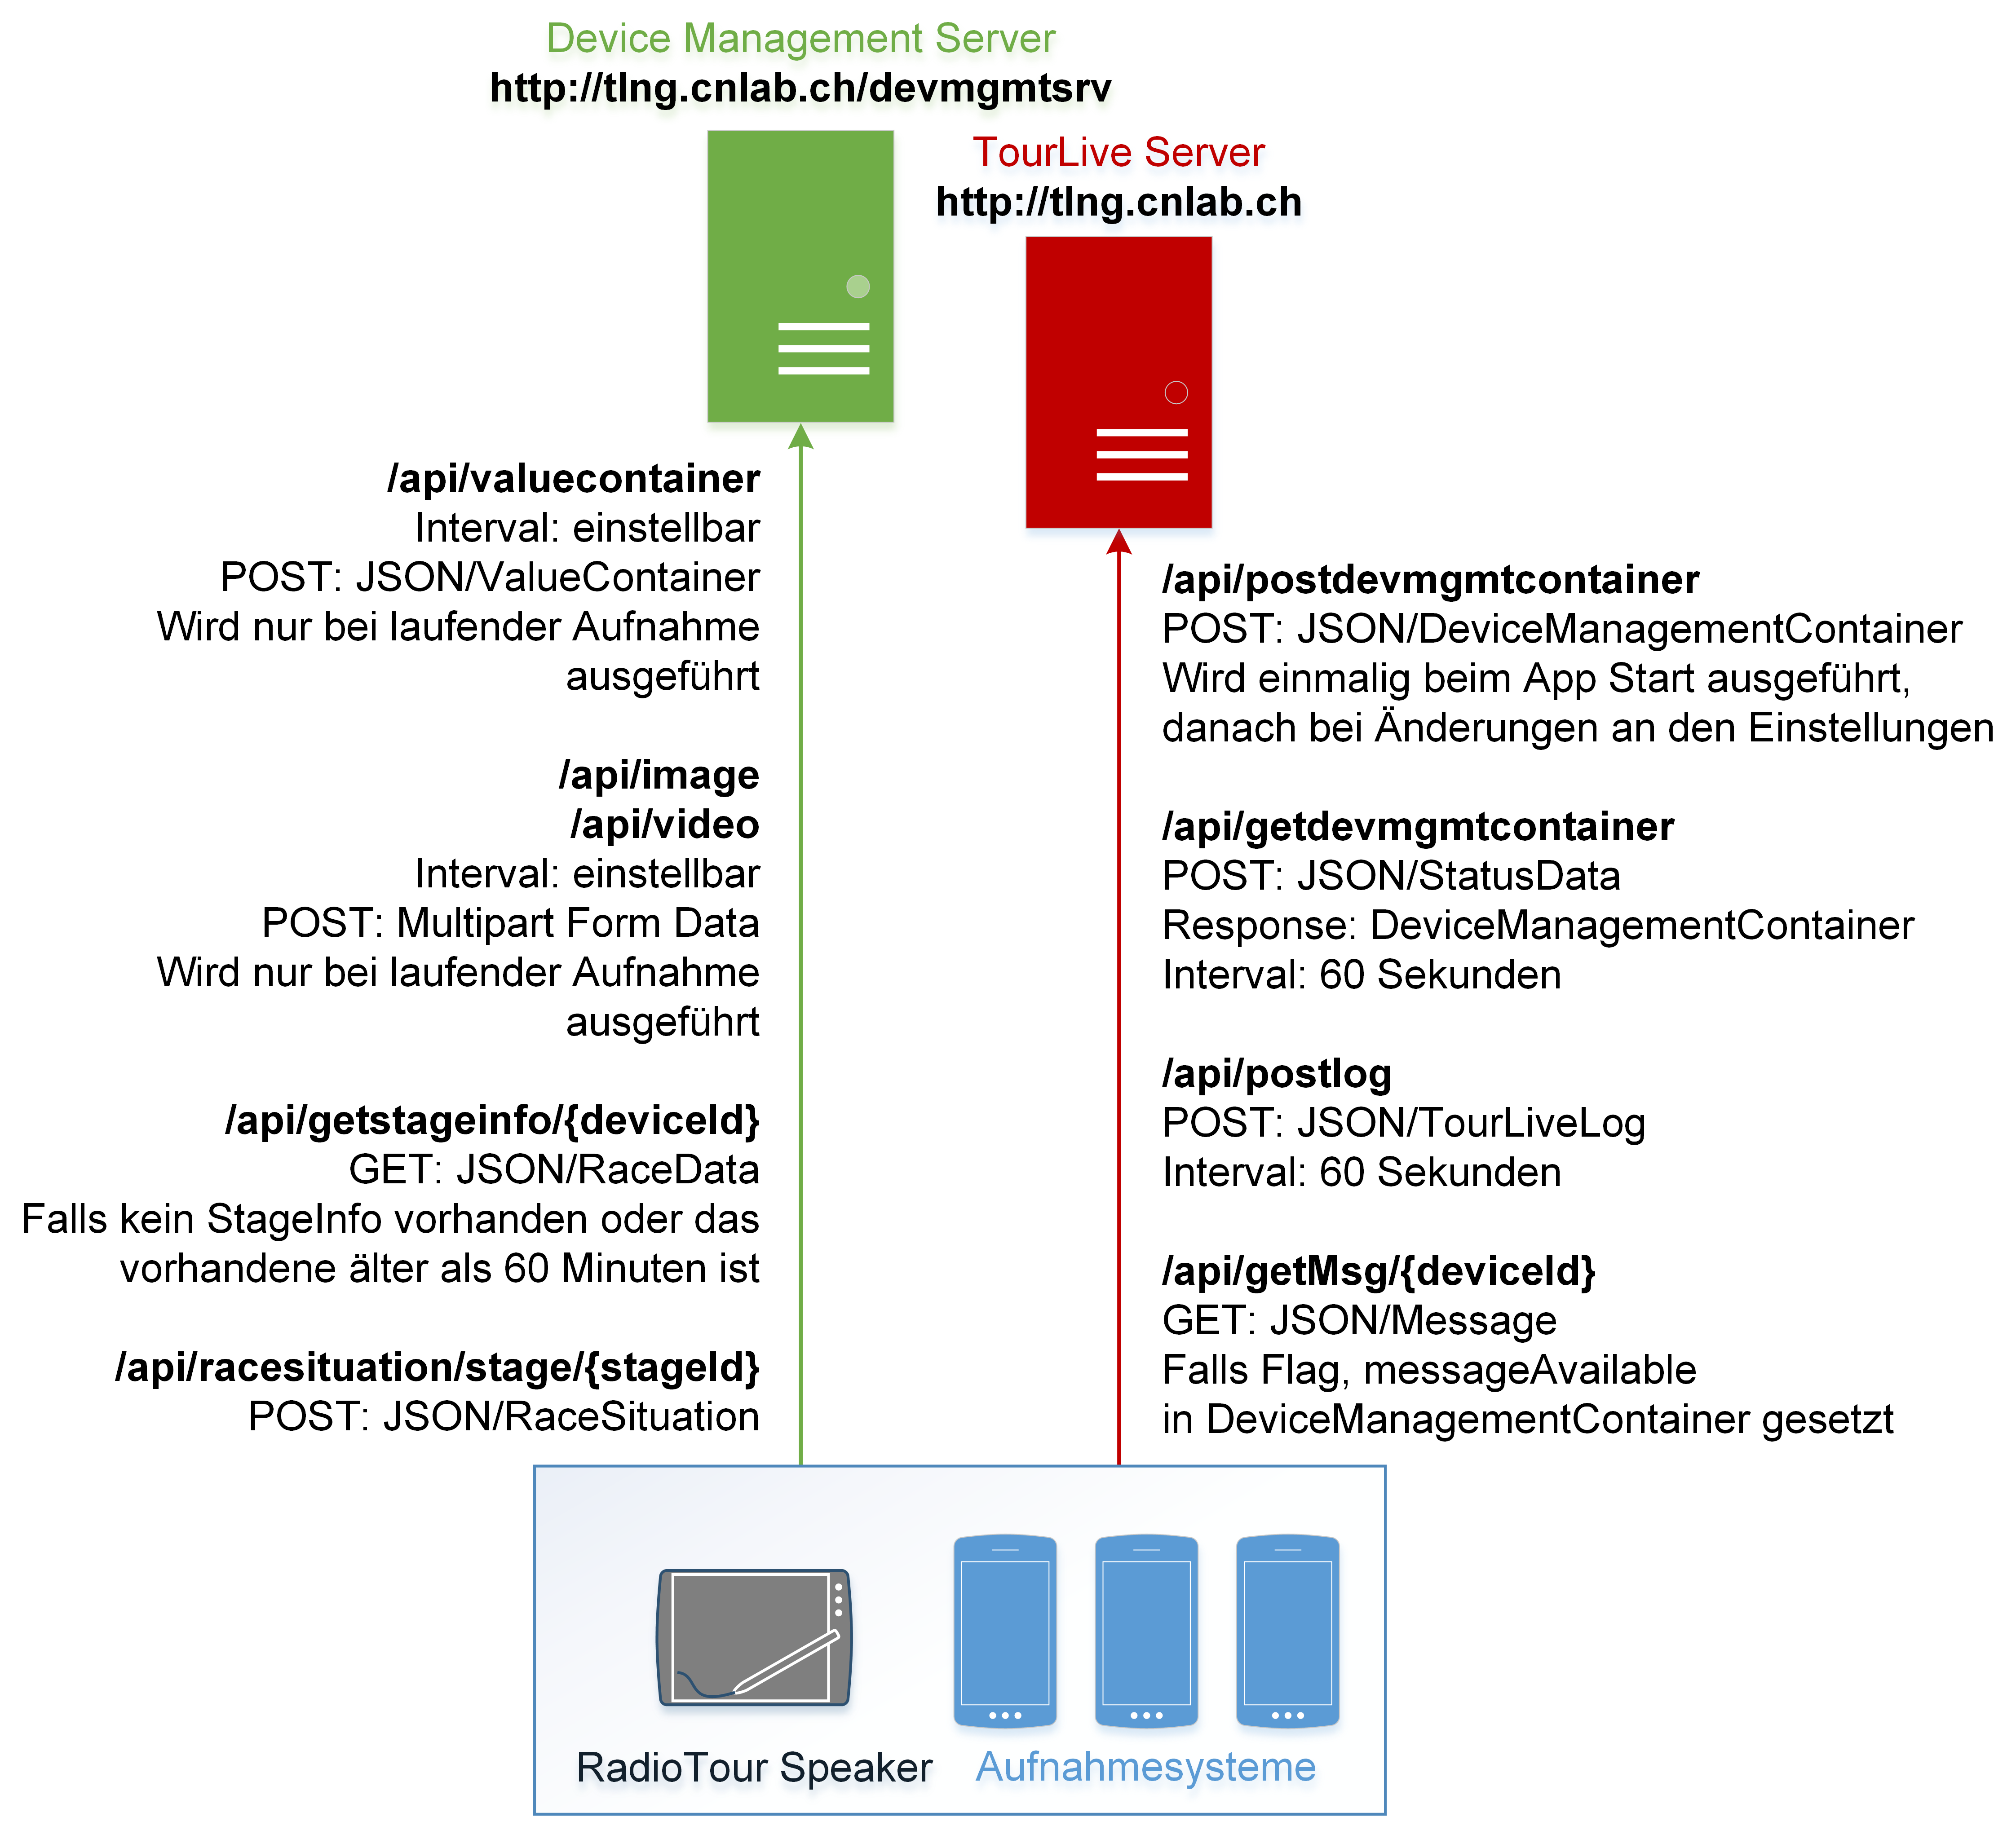
\includegraphics[width=130mm]{images/uebersicht_schnittstelle.png}
	\caption{Übersicht Schnittstellen}
\end{figure}

\section{TourLive Interne Schnittstelle}
\label{sec:tourliveserverapi}
Die Aufnahmegeräte liefern an dieser Stelle die ValueContainer, Bilder und Videos dem TourLive Server, dies wird als die interne Schnittstelle (\textit{\gls{api}}) bezeichnet. Die benötigten Felder sind jeweils im Bereich \textit{Request} erkennbar.

\subsection{ValueContainer posten}
\begin{longtable}{ p{2.5cm} p{3.5cm} p{6cm}}
	\textbf{URL:} & \multicolumn{2}{p{10cm}}{/api/valuecontainer} \\
	\textbf{Request:} & Method: & POST \\
		& Content-Type: & application/json \\
		& Body: & JSON-String 'ValueContainer'\\
	\textbf{Response:} & Header: & HTTP/1.1 200 OK \\
		& Body: & <empty> \\
	\textbf{Zeitpunkt:} & \multicolumn{2}{p{10cm}}{Bei laufender Aufnahme} \\ 
	\textbf{Interval:} & \multicolumn{2}{p{10cm}}{einstellbar} \\ 
	\caption{Schnittstelle ValueContainer}
\end{longtable}

\subsubsection{ValueContainer JSON}
\begin{figure}[H]
	\centering
	\lstinputlisting[language=json]{jsonfiles/valueContainer.json}
	\caption{ValueContainer JSON}
	\label{fig:valuecontainer}
\end{figure}

\subsection{Image posten}
\begin{longtable}{ p{2.5cm} p{3.5cm} p{6cm}}
	\textbf{URL:} & \multicolumn{2}{p{10cm}}{/api/image} \\
	\textbf{Request:} & Method: & POST \\
		& Content-Type: & multipart/form-data [3 Boundaries] \\
		& Body-Boundary 1: & text/plain (timestamp) \\
		& Body-Boundary 2: & text/plain (deviceId) \\
		& Body-Boundary 3: & application/octet-stream (Bild) \\
	\textbf{Response:} & Header: & HTTP/1.1 200 OK \\
		& Body: & <empty> \\
	\textbf{Zeitpunkt:} & \multicolumn{2}{p{10cm}}{Bei laufender Aufnahme, falls Image aktiviert ist} \\ 
	\textbf{Interval:} & \multicolumn{2}{p{10cm}}{einstellbar}
\end{longtable}

\subsection{Video posten}
\begin{longtable}{ p{2.5cm} p{3.5cm} p{6cm}}
	\textbf{URL:} & \multicolumn{2}{p{10cm}}{/api/video} \\
	\textbf{Request:} & Method: & POST \\
		& Content-Type: & multipart/form-data [3 Boundaries] \\
		& Body-Boundary 1: & text/plain (timestamp) \\
		& Body-Boundary 2: & text/plain (deviceId) \\
		& Body-Boundary 3: & application/octet-stream (Video) \\
	\textbf{Response:} & Header: & HTTP/1.1 200 OK \\
		& Body: & <empty> \\
	\textbf{Zeitpunkt:} & \multicolumn{2}{p{10cm}}{Bei laufender Aufnahme, falls der Videostream aktiviert ist} \\ 
	\textbf{Interval:} & \multicolumn{2}{p{10cm}}{einstellbar} 
\end{longtable}

\subsection{RaceSituation posten}
\begin{longtable}{ p{2.5cm} p{3.5cm} p{6cm}}
	\textbf{URL:} & \multicolumn{2}{p{10cm}}{/api/racesituation/stage/\{stageId\}} \\
	\textbf{Request:} & Method: & POST \\
		& Body: & JSON-String 'RaceSituation'\\	
	\textbf{Response:} & Header: & HTTP/1.1 200 OK \\
		& Body: & <empty> \\	
	\textbf{Bemerkung:} & \multicolumn{2}{p{10cm}}{Der RadioTourSpeaker sendet (unabhängig von den TourLive Aufnahmegeräten) periodisch die Rennsituation an den Server}
\end{longtable}

\subsubsection{RaceSituation JSON}
Der TourLive Server erwartet das folgende JSON für die Darstellung der Rennsituation.
\begin{figure}[H]
	\centering
	\lstinputlisting[language=json]{jsonfiles/raceSituation.json}
	\caption{RaceSituation JSON}
\end{figure}


\subsection{StageInfo abfragen}
\begin{longtable}{ p{2.5cm} p{3.5cm} p{6cm}}
	\textbf{URL:} & \multicolumn{2}{p{10cm}}{/api/getstageinfo/\{deviceId\}} \\
	\textbf{Request:} & Method: & GET \\
		& Body: & <empty>\\	
	\textbf{Response:} & Header: & HTTP/1.1 200 OK \\
		& Content-Type: & application/json \\
		& Body: & Custom JSON-String \\	
	\textbf{Bemerkung:} & \multicolumn{2}{p{10cm}}{Im Body der Response wird eine eigens kreierte HashMap ausgeliefert, darin sind aktuelle Etappeninformationen für das angegebene Gerät. Diese Informationen werden für den Rennbegleiter auf dem Gerät dargestellt} \\ [1ex] 
\caption{Schnittstellen StageInfo}
\end{longtable}

\subsection{StageInfo JSON}
\begin{figure}[H]
	\centering
	\lstinputlisting[language=json]{jsonfiles/stageInfo.json}
	\caption{StageInfo JSON}
\end{figure}


\section{TourLive Public API}
\label{sec:tourlivepublicapi}
Die Renn- und Etappeninformationen stehen für Drittentwickler zur Verfügung. Zu jeder Etappe können zusätzlich die ValueContainer und Bilddaten abgefragt werden.

\subsection{Etappen abfragen}
\begin{longtable}{ p{2.5cm} p{3.5cm} p{6cm}}
	\textbf{URL:} & \multicolumn{2}{l}{/public/stages} \\
	\textbf{Request:} & Method: & GET \\
		& Body: & <empty>\\
	\textbf{Response:} &  Header: & HTTP/1.1 200 OK \\
		& Content-Type: & application/json \\
		& Body: & JSON-Array 'Stages'\\
	\textbf{Bemerkung:} & \multicolumn{2}{p{10cm}}{Alle sichtbaren Etappen} 
\end{longtable}
\subsubsection{Etappen JSON}
\begin{figure}[H]
	\centering
	\lstinputlisting[language=json]{jsonfiles/stages.json}
	\caption{Etappen JSON}
\end{figure}

\subsection{ValueContainer abfragen}
\begin{longtable}{ p{2.5cm} p{3.5cm} p{6cm}}
	\textbf{URL:} & \multicolumn{2}{l}{/public/stage/\{stageId\}/valuecontainer} \\
	\textbf{Request:} & Method: & GET \\
		& Body: & <empty>\\
	\textbf{Response:} &  Header: & HTTP/1.1 200 OK \\
		& Content-Type: & application/json \\
		& Body: & JSON-Array 'ValueContainers'\\
	\textbf{Bemerkung:} & \multicolumn{2}{p{10cm}}{Alle ValueContainers einer Etappe}
\end{longtable}

\subsection{ImageData abfragen}
\begin{longtable}{ p{2.5cm} p{3.5cm} p{6cm}}
	\textbf{URL:} & \multicolumn{2}{l}{/public/stage/\{stageId\}/imagedata} \\
	\textbf{Request:} & Method: & GET \\
		& Body: & <empty>\\
	\textbf{Response:} &  Header: & HTTP/1.1 200 OK \\
		& Content-Type: & application/json \\
		& Body: & JSON-Array 'ImageData'\\
	\textbf{Bemerkung:} & \multicolumn{2}{p{10cm}}{Alle ImageData Objekte zu dieser Etappe, nicht aber die eigentlichen Bilder. Die Bilder können aber mit dem Feld \textit{imageLocation} entweder direkt verlinkt oder heruntergeladen werden}
\end{longtable}

\subsubsection{ImageData JSON}
\begin{figure}[H]
	\centering
	\lstinputlisting[language=json]{jsonfiles/imageData.json}
	\caption{ImageData JSON}
\end{figure}

\subsection{VideoData abfragen}	
\begin{longtable}{ p{2.5cm} p{3.5cm} p{6cm}}
	\textbf{URL:} & \multicolumn{2}{l}{/public/stage/\{stageId\}/videodata} \\
	\textbf{Request:} & Method: & GET \\
		& Body: & <empty>\\
	\textbf{Response:} &  Header: & HTTP/1.1 200 OK \\
		& Content-Type: & application/json \\
		& Body: & JSON-Array 'VideoData'\\
	\textbf{Bemerkung:} & \multicolumn{2}{p{10cm}}{Alle VideoData Objekte zu dieser Etappe, nicht aber die eigentlichen Videosequenzen. Die Videos können aber mit dem Feld \textit{videoLocation} entweder direkt verlinkt oder heruntergeladen werden}
\end{longtable}

\subsection{MarchTableItem abfragen}
\begin{longtable}{ p{2.5cm} p{3.5cm} p{6cm}}
	\textbf{URL:} & \multicolumn{2}{l}{/public/stage/\{stageId\}/marchtableitem} \\
	\textbf{Request:} & Method: & GET \\
		& Body: & <empty>\\
	\textbf{Response:} &  Header: & HTTP/1.1 200 OK \\
		& Content-Type: & application/json \\
		& Body: & JSON-Array 'MarchTableItem'\\
	\textbf{Bemerkung:} & \multicolumn{2}{p{10cm}}{Die Marschtabelle ist aufgeteilt in Einheiten. Jede Reihe bedeutet eine Einheit. Pro Etappe können alle Marschtabelleneinheiten abgerufen werden.}
\end{longtable}

\subsubsection{MarchTableItem abfragen}
\begin{figure}[H]
	\centering
	\lstinputlisting[language=json]{jsonfiles/marchTableItems.json}
	\caption{MarchTableItem JSON}
\end{figure}

\subsection{Riders abfragen}
\begin{longtable}{ p{2.5cm} p{3.5cm} p{6cm}}	
	\textbf{URL:} & \multicolumn{2}{l}{/public/stage/\{stageId\}/riders} \\
	\textbf{Request:} & Method: & GET \\
		& Body: & <empty>\\
	\textbf{Response:} &  Header: & HTTP/1.1 200 OK \\
		& Content-Type: & application/json \\
		& Body: & JSON-Array 'Riders'\\
	\textbf{Bemerkung:} & \multicolumn{2}{p{10cm}}{Sämtliche Fahrer, welche dieser Etappe zugeordnet sind} \\ [1ex] 
\caption{TourLive Public API}
\end{longtable}

\subsubsection{Riders JSON}
\begin{figure}[H]
	\centering
	\lstinputlisting[language=json]{jsonfiles/riders.json}
	\caption{Riders JSON}
\end{figure}

\section{Device Management Portal Schnittstelle}

\subsection{Einstellungen posten}
Sobald die Einstellungen in der App geändert werden, müssen sie über diese Schnittstelle an den Server gesendet werden.

{\renewcommand{\arraystretch}{1}
    \begin{longtable}{ p{2.5cm} p{3.5cm} p{6cm}}
	\textbf{URL:} & \multicolumn{2}{l}{/devmgmtsrv/api/postdevmgmtsrv} \\
	\textbf{Request:} & Method: & POST \\
		& Content-Type: & application/json \\
		& Body: & JSON-String 'DeviceManagementContainer'\\
	\textbf{Response:} &  Header: & HTTP/1.1 200 OK \\
		& Body: & <empty>	\\
	\textbf{Eigenschaft:} & \multicolumn{2}{p{10cm}}{Wird einmalig beim App Start ausgeführt sowie bei lokalen Änderungen in den Einstellungen} \\
	\textbf{Interval:} & \multicolumn{2}{p{10cm}}{unregelmässig} \\
	
\caption{Schnittstelle Einstellungen}
\end{longtable}}

\subsubsection{Einstellungen JSON}
\begin{figure}[H]
	\centering
	\lstinputlisting[language=json]{jsonfiles/settings.json}
	\caption{Einstellungen JSON}
\end{figure}

\subsection{Status posten und Einstellungen erhalten}

Um den aktuellen Status des Aufnahmesystems dem Server mitzuteilen kann diese Methode aufgerufen werden. Als Antwort erhält man die im Moment aktuellen Einstellungen.

{\renewcommand{\arraystretch}{1}
    \begin{longtable}{ p{2.5cm} p{3.5cm} p{6cm}} 
	\textbf{URL:} & \multicolumn{2}{l}{/devmgmtsrv/api/getdevmgmtsrv} \\
	\textbf{Request:} & Content-Type: & application/json \\
		& Method: & POST \\
		& Body: & JSON-String 'StatusData' \\
	\textbf{Response:} & Method: & POST \\
		& Content-Type: & application/json \\
		& Body: & JSON-String 'DeviceManagementContainer' \\
	\textbf{Eigenschaft:} & \multicolumn{2}{p{10cm}}{Wird regelmässig als Service ausgeführt.} \\ 
	\textbf{Interval:} & \multicolumn{2}{p{10cm}}{regelmässig - alle 60 Sekunden} \\
	
\caption{Schnittstelle Status}
\end{longtable}	}
\subsubsection{Status JSON}

Das JSON eines Status Posts sieht folgendermassen aus:

\begin{figure}[H]
	\centering
	\lstinputlisting[language=json]{jsonfiles/status.json}
	\caption{Status JSON}
\end{figure}


\subsection{Log posten}

Um neue Logeinträge dem Server zu übermitteln kann diese Methode benutzt werden.

{\renewcommand{\arraystretch}{1}
    \begin{longtable}{ p{2.5cm} p{3.5cm} p{6cm}}
	\textbf{URL:} & \multicolumn{2}{p{10cm}}{/devmgmtsrv/api/postlog} \\
	\textbf{Request:} & Method: & POST \\
		& Content-Type: & application/json \\
		& Body: & JSON-String 'TourLiveLog' \\
	\textbf{Response:} &  Header: & HTTP/1.1 200 OK \\
		& Body: & <empty>	\\
	\textbf{Eigenschaft:} &  \multicolumn{2}{p{10cm}}{Wird regelmässig als Service ausgeführt.}\\ 
	\textbf{Interval:} &  \multicolumn{2}{p{10cm}}{regelmässig - alle 60 Sekunden}\\
	
\caption{Schnittstelle Log}
\end{longtable}}

\subsubsection{Log JSON}

Das JSON eines Log Posts sieht folgendermassen aus:

\begin{figure}[H]
	\centering
	\lstinputlisting[language=json]{jsonfiles/log.json}
	\caption{Log JSON}
\end{figure}

\subsection{Nachricht abholen}

Sofern eine neue Nachricht für das Gerät vorhanden ist kann sie über diese Methoden abgeholt werden.

{\renewcommand{\arraystretch}{1}
    \begin{longtable}{ p{2.5cm} p{3.5cm} p{6cm}}

	\textbf{URL:} & \multicolumn{2}{p{10cm}}{/devmgmtsrv/api/getMsg/\{deviceId\}} \\
	\textbf{Request:} & Method: & GET \\
		& Body: & <empty> \\
	\textbf{Response:} & Method: & POST \\
		& Content-Type: & application/json \\
		& Body: & JSON-String 'Message' \\
	\textbf{Eigenschaft:} & \multicolumn{2}{p{10cm}}{ Wenn das 'messageAvailable'-Flag gesetzt ist in einem empfangenen DeviceManagementContainer.} \\
	\textbf{Interval:} & \multicolumn{2}{p{10cm}}{unregelmässig}\\
	
\caption{Schnittstelle Nachricht abholen}
\end{longtable} }

\subsubsection{Nachrichten JSON}
Das JSON für die Nachrichten ist das folgende:
\begin{figure}[H]
	\centering
	\lstinputlisting[language=json]{jsonfiles/message.json}
	\caption{Nachrichten JSON}
\end{figure}


